% Chapter Template

\chapter{Methods} % Main chapter title

\label{Chapter2} % Change X to a consecutive number; for referencing this chapter elsewhere, use \ref{ChapterX}

%----------------------------------------------------------------------------------------
%	SECTION 1
%----------------------------------------------------------------------------------------

\section{Reynolds Number}

Our first goal is to identify a set of points of interest. Because turbulent flow is where we need to study, we need to calculate the Reynolds-Number (\ensuremath{RE}) of each voxel in every time step of the simulation. We take the product of \ensuremath{p, u} and \ensuremath{L} where \ensuremath{p} is the density of the fluid, \ensuremath{u} is the flow speed of the fluid, and \ensuremath{L} is the characteristic linear dimension. Then using the dynamic viscosity of fluid represented as µ as the divisor to get the \ensuremath{RE} for that voxel in that time-step(Eqn. \ref{eq:1}). It should be noted that for consistency in our simulations L is calculated from the average length of the sides of each voxel (\ensuremath{\sqrt[3]{length * width * height}}). Due to the scale being a constant in each calculation, changing this value can affect the scale of values obtained, but it does not alter the distribution of the values. 


\begin{equation}\label{eq:1}
RE  = \frac{puL} {\mu} 
\end{equation}


Now we have the Reynolds Number of every voxel in each time-step \ensuremath{RE_t} where \ensuremath{t} is an index number referencing a time value. Next, we find the mean value for each voxel \ref{eq:2} then threshold the data into two categories; \ensuremath{RE >= 150} as turbulent flow and \ensuremath{0 < RE <= 40} as laminar flow. We exclude \ensuremath{RE} values of zero because they are indicative of a voxel that is within an obstruction (e.g. underground, inside of a tree). Next we RE threshold our 3-D points in space to locate points of interest.


\begin{equation} \label{eq:2}
\langle RE\rangle_{mean} = \frac{1}{T} \sum_{t=1}^{T} RE_{t}=\frac{1}{T}\left(RE_{1}+\cdots+RE_{T}\right)
\end{equation} 

Because the number of voxels with \ensuremath{\langle RE\rangle} greater than the threshold is large we run a clustering algorithm on voxels with \ensuremath{\langle RE\rangle} above the threshold, in this case we use k-means due to its ease of implementation and speed when clustering large sets of points \cite{HDBScan}. This groups all points into \ensuremath{k} groups while minimizing the distance between a point and that group’s centroid. We calculate the value of \ensuremath{k} by taking the \ensuremath{\frac{1}{2}\sqrt[3]{I*J*K}} where \ensuremath{I,J} and \ensuremath{K} are the number of voxels in the \ensuremath{x}, \ensuremath{y} and \ensuremath{z} axis respectively. We then are able to take the centroid from each cluster and refer to these as our points of interest reducing the points of interest by approximately 7000.




\begin{figure}
\centering
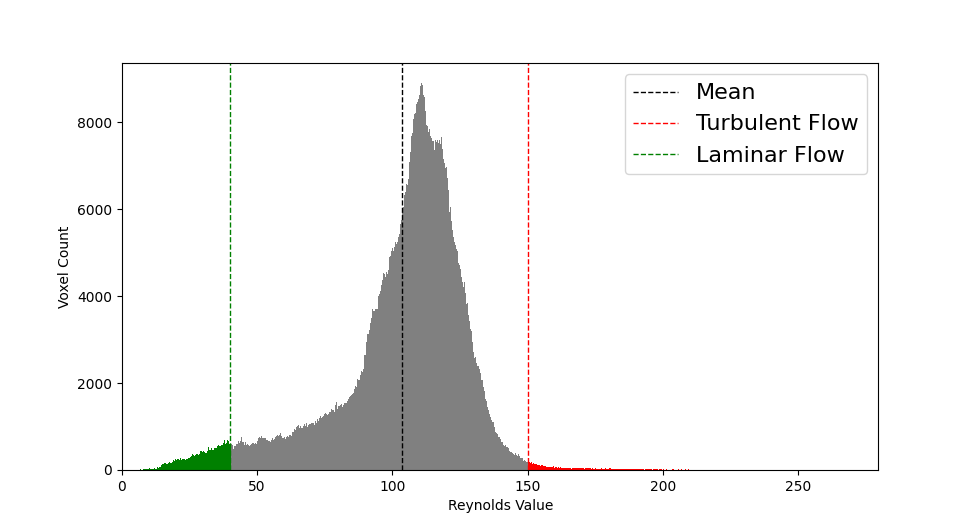
\includegraphics[scale=.35]{Figures/Hist4_11.png}
\decoRule
\caption[Reynolds Number Histogram]{Mean Reynolds Values Histogram}
\label{fig:MHistgram}
\end{figure}

\begin{figure}
\centering
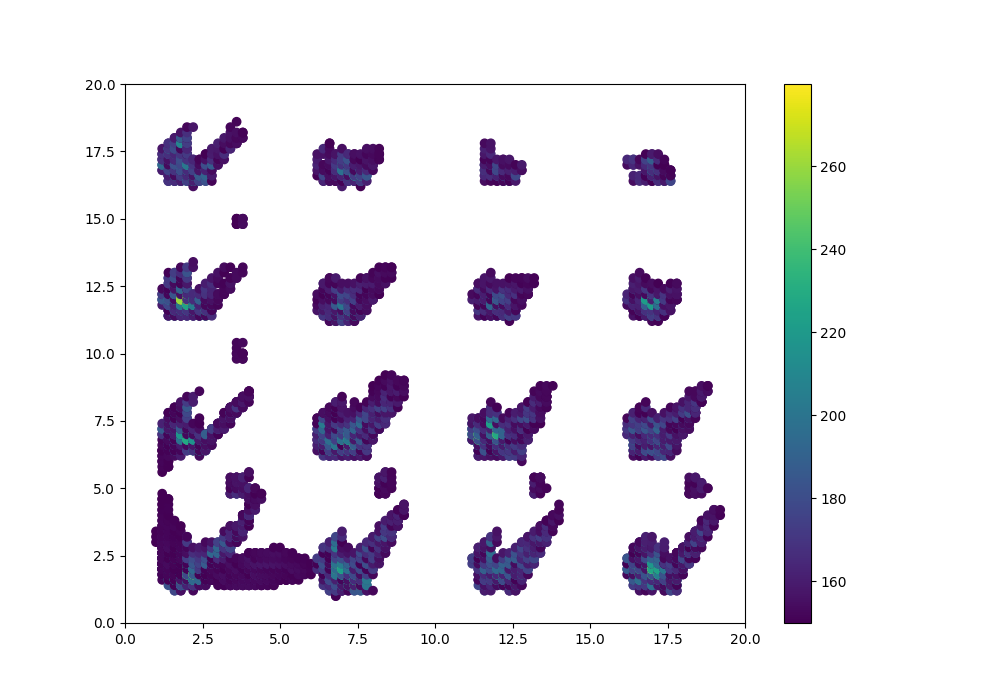
\includegraphics[scale=.35]{Figures/Turb2D_4_11.png}
\decoRule
\caption[Turbulent Air Flow Scatter Plot]{A top down view of a plot showing areas of turbulent air flow containing 7705 points}
\label{fig:MTurbulentflow}
\end{figure}
%-----------------------------------
%	SECTION 2
%-----------------------------------
\section{Pathline Calculations}

Now that we have calculated the points of interest we can use an Ordinary Differential Equation solver to calculate the streamlines. We will use a fifth-order Runge-Kutta method for adaptive time steps and to minimize errors in calculations \cite{Teitzel1997}. We are able to use forward and reverse integration to calculate pathlines for every time step that passes through these points of interest. After integrating in both directions we then combine the posting and time data for each pathline while also adding in the Reynolds Number for each point as well. We chose to store all of this data in hdf5 formatting so it can be efficiently loaded in parallel into our visualization pipeline\cite{hdf5}. [Fol+11] 



%-----------------------------------
%	SECTION 3
%-----------------------------------
\section{Unity Visualization}

Once we read in pathline and scene data into Unity, we determine the largest (\ensuremath{REmax}) and smallest (\ensuremath{REmin}) value within the data set. Now having the minimum and maximum values we are able to calculate a color value for each segment of the pathlines. To do so we have to calculate the interpolant value within the range [\ensuremath{REmin, REmax}] (Eqn. \ref{eq:3}). This provides us with a value between [0,1] allowing us to  map this value to a color on a perceptually uniform color map. We selected Vega’s magma color map with eight colors\cite{colorschemes}. For each time step, we load in the respective data for all \ensuremath{k} pathlines. To resolve the issue of being able to see orientation but not true directionality of a pathline we segment each pathline into n-1 line segments (e.g. \ensuremath{P_0\rightarrow P_1},\ensuremath{P_1 \rightarrow P_2}, ... ,\ensuremath{P_{n-2} \rightarrow P_{n-1}}).
We then adjust the starting width of each line segment to be the average length of a voxel and the ending width zero. Figure \ref{fig:UnityPathline} illustrates the benefits of this visual change. Using cones resolves the issues with direction of pathlines as previously discussed. We then build a color gradient texture and apply it to the texture from point to point with the precalculated color map. We are able to compile and build our Unity system into an executable file that allows for the end user to run on any compatible system. We have the user interface (UI) designed to allow for viewing the simulation using a Head Mounted Display (HMD), a virtual reality headset, and controller or a computer monitor with a keyboard and mouse for movement. Users just need to type in the directory of the hdf5 files output discussed previously and the data is cached for quick loading into the simulation. Users are then able to move around the environment in either Virtual Reality or just by using the mouse and keyboard. 


\begin{equation} \label{eq:3}
f(RE_{min},RE_{max},RE_{value}) = \frac{RE_{value}-RE_{min}}{RE_{max}-RE_{min}}
\end{equation} 

\begin{figure}
\centering
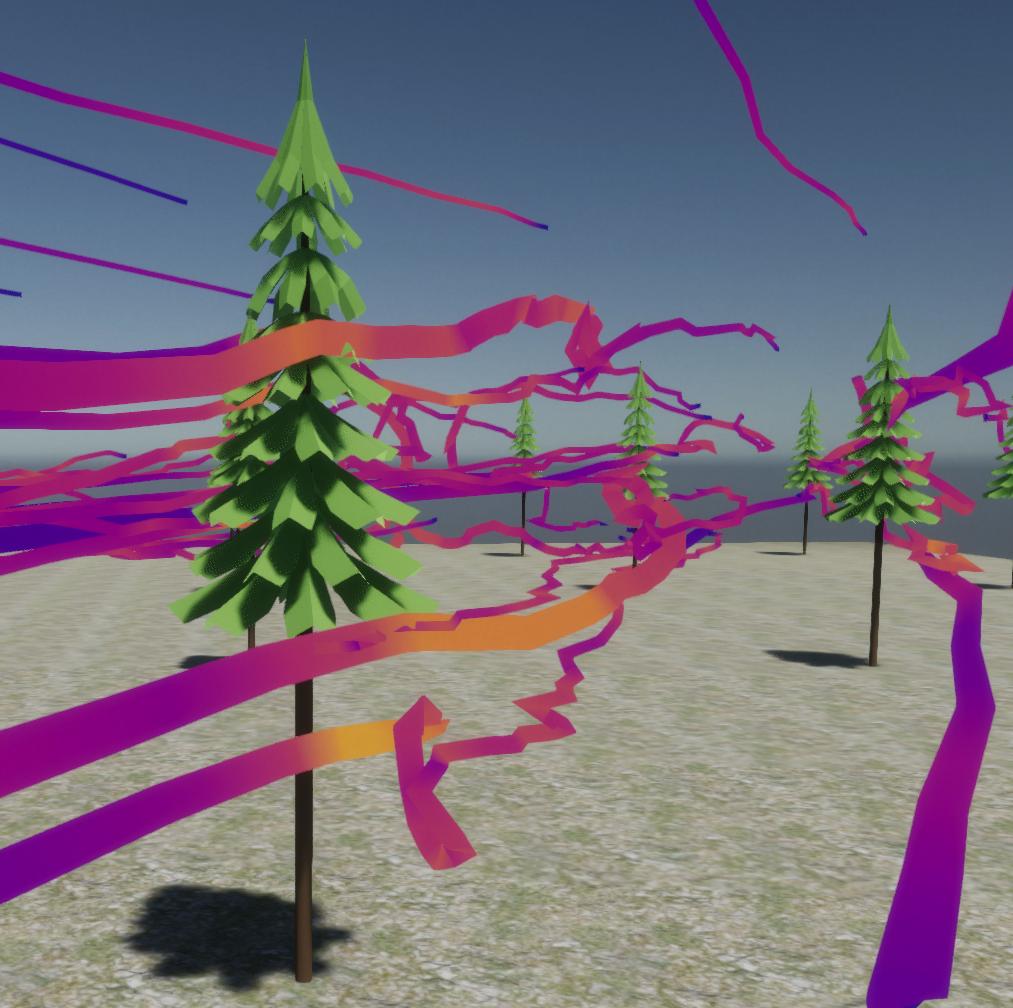
\includegraphics[scale=.3]{Figures/TreePathline1.png}
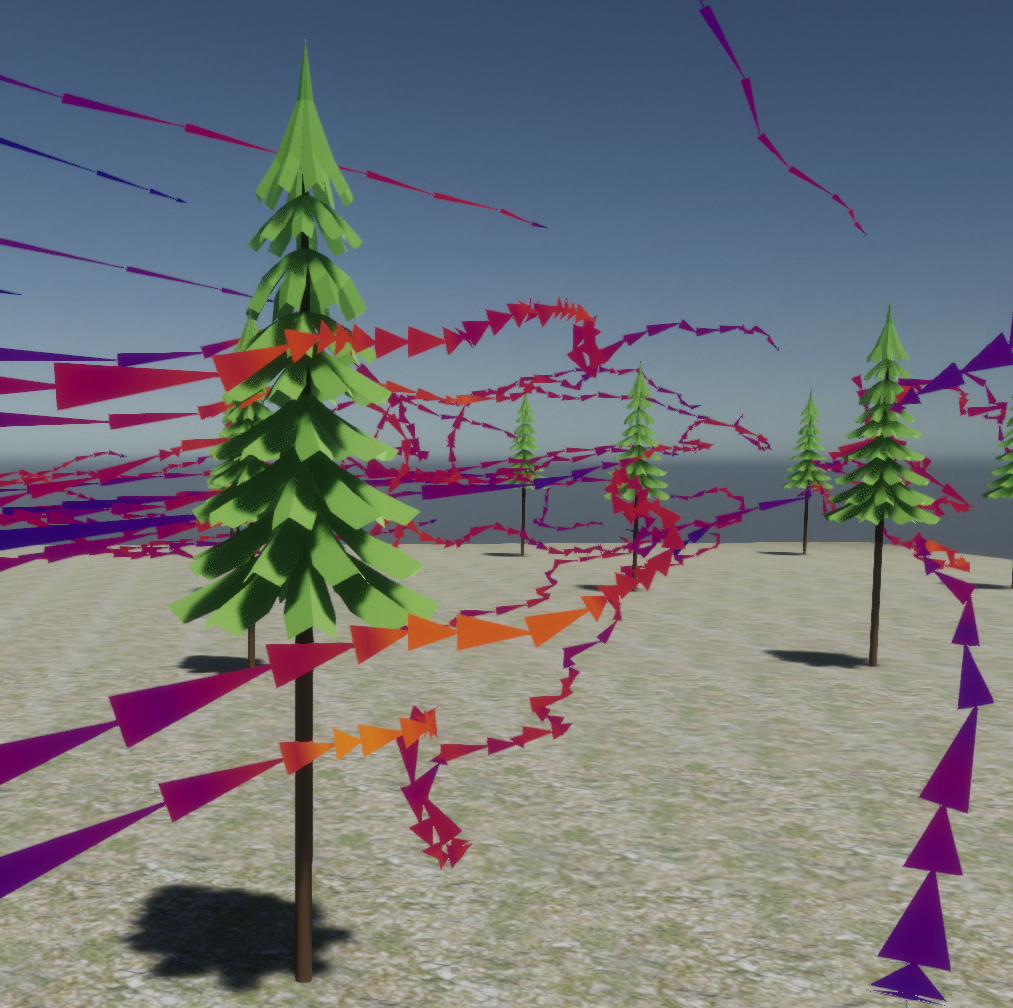
\includegraphics[scale=.3]{Figures/TreePathline2.png}
\decoRule
\caption[Pathlines comparisons in Unity]{\textbf{Top:} Pathlines visualized as a single line  \textbf{Bottom:} Pathlines broken in to line segments }
\label{fig:UnityPathline}
\end{figure}
